\PassOptionsToPackage{unicode=true}{hyperref} % options for packages loaded elsewhere
\PassOptionsToPackage{hyphens}{url}
%
\documentclass[10pt,ignorenonframetext,]{beamer}
\usepackage{pgfpages}
\setbeamertemplate{caption}[numbered]
\setbeamertemplate{caption label separator}{: }
\setbeamercolor{caption name}{fg=normal text.fg}
\beamertemplatenavigationsymbolsempty
% Prevent slide breaks in the middle of a paragraph:
\widowpenalties 1 10000
\raggedbottom
\setbeamertemplate{part page}{
\centering
\begin{beamercolorbox}[sep=16pt,center]{part title}
  \usebeamerfont{part title}\insertpart\par
\end{beamercolorbox}
}
\setbeamertemplate{section page}{
\centering
\begin{beamercolorbox}[sep=12pt,center]{part title}
  \usebeamerfont{section title}\insertsection\par
\end{beamercolorbox}
}
\setbeamertemplate{subsection page}{
\centering
\begin{beamercolorbox}[sep=8pt,center]{part title}
  \usebeamerfont{subsection title}\insertsubsection\par
\end{beamercolorbox}
}
\AtBeginPart{
  \frame{\partpage}
}
\AtBeginSection{
  \ifbibliography
  \else
    \frame{\sectionpage}
  \fi
}
\AtBeginSubsection{
  \frame{\subsectionpage}
}
\usepackage{lmodern}
\usepackage{setspace}
\setstretch{1.0}
\usepackage{amssymb,amsmath}
\usepackage{ifxetex,ifluatex}
\usepackage{fixltx2e} % provides \textsubscript
\ifnum 0\ifxetex 1\fi\ifluatex 1\fi=0 % if pdftex
  \usepackage[T1]{fontenc}
  \usepackage[utf8]{inputenc}
  \usepackage{textcomp} % provides euro and other symbols
\else % if luatex or xelatex
  \usepackage{unicode-math}
  \defaultfontfeatures{Ligatures=TeX,Scale=MatchLowercase}
\fi
\usetheme[]{CambridgeUS}
\usefonttheme{serif}
% use upquote if available, for straight quotes in verbatim environments
\IfFileExists{upquote.sty}{\usepackage{upquote}}{}
% use microtype if available
\IfFileExists{microtype.sty}{%
\usepackage[]{microtype}
\UseMicrotypeSet[protrusion]{basicmath} % disable protrusion for tt fonts
}{}
\IfFileExists{parskip.sty}{%
\usepackage{parskip}
}{% else
\setlength{\parindent}{0pt}
\setlength{\parskip}{6pt plus 2pt minus 1pt}
}
\usepackage{hyperref}
\hypersetup{
            pdftitle={Título do meu relatório (html\_pdf\_document)},
            pdfauthor={Cristian Villegas (clobos@usp.br)},
            pdfborder={0 0 0},
            breaklinks=true}
\urlstyle{same}  % don't use monospace font for urls
\newif\ifbibliography
\usepackage{color}
\usepackage{fancyvrb}
\newcommand{\VerbBar}{|}
\newcommand{\VERB}{\Verb[commandchars=\\\{\}]}
\DefineVerbatimEnvironment{Highlighting}{Verbatim}{commandchars=\\\{\}}
% Add ',fontsize=\small' for more characters per line
\usepackage{framed}
\definecolor{shadecolor}{RGB}{42,33,28}
\newenvironment{Shaded}{\begin{snugshade}}{\end{snugshade}}
\newcommand{\AlertTok}[1]{\textcolor[rgb]{1.00,1.00,0.00}{#1}}
\newcommand{\AnnotationTok}[1]{\textcolor[rgb]{0.00,0.40,1.00}{\textbf{\textit{#1}}}}
\newcommand{\AttributeTok}[1]{\textcolor[rgb]{0.74,0.68,0.62}{#1}}
\newcommand{\BaseNTok}[1]{\textcolor[rgb]{0.27,0.67,0.26}{#1}}
\newcommand{\BuiltInTok}[1]{\textcolor[rgb]{0.74,0.68,0.62}{#1}}
\newcommand{\CharTok}[1]{\textcolor[rgb]{0.02,0.61,0.04}{#1}}
\newcommand{\CommentTok}[1]{\textcolor[rgb]{0.00,0.40,1.00}{\textbf{\textit{#1}}}}
\newcommand{\CommentVarTok}[1]{\textcolor[rgb]{0.74,0.68,0.62}{#1}}
\newcommand{\ConstantTok}[1]{\textcolor[rgb]{0.74,0.68,0.62}{#1}}
\newcommand{\ControlFlowTok}[1]{\textcolor[rgb]{0.26,0.66,0.93}{\textbf{#1}}}
\newcommand{\DataTypeTok}[1]{\textcolor[rgb]{0.74,0.68,0.62}{\underline{#1}}}
\newcommand{\DecValTok}[1]{\textcolor[rgb]{0.27,0.67,0.26}{#1}}
\newcommand{\DocumentationTok}[1]{\textcolor[rgb]{0.00,0.40,1.00}{\textit{#1}}}
\newcommand{\ErrorTok}[1]{\textcolor[rgb]{1.00,1.00,0.00}{\textbf{#1}}}
\newcommand{\ExtensionTok}[1]{\textcolor[rgb]{0.74,0.68,0.62}{#1}}
\newcommand{\FloatTok}[1]{\textcolor[rgb]{0.27,0.67,0.26}{#1}}
\newcommand{\FunctionTok}[1]{\textcolor[rgb]{1.00,0.58,0.35}{\textbf{#1}}}
\newcommand{\ImportTok}[1]{\textcolor[rgb]{0.74,0.68,0.62}{#1}}
\newcommand{\InformationTok}[1]{\textcolor[rgb]{0.00,0.40,1.00}{\textbf{\textit{#1}}}}
\newcommand{\KeywordTok}[1]{\textcolor[rgb]{0.26,0.66,0.93}{\textbf{#1}}}
\newcommand{\NormalTok}[1]{\textcolor[rgb]{0.74,0.68,0.62}{#1}}
\newcommand{\OperatorTok}[1]{\textcolor[rgb]{0.74,0.68,0.62}{#1}}
\newcommand{\OtherTok}[1]{\textcolor[rgb]{0.74,0.68,0.62}{#1}}
\newcommand{\PreprocessorTok}[1]{\textcolor[rgb]{0.74,0.68,0.62}{\textbf{#1}}}
\newcommand{\RegionMarkerTok}[1]{\textcolor[rgb]{0.74,0.68,0.62}{#1}}
\newcommand{\SpecialCharTok}[1]{\textcolor[rgb]{0.02,0.61,0.04}{#1}}
\newcommand{\SpecialStringTok}[1]{\textcolor[rgb]{0.02,0.61,0.04}{#1}}
\newcommand{\StringTok}[1]{\textcolor[rgb]{0.02,0.61,0.04}{#1}}
\newcommand{\VariableTok}[1]{\textcolor[rgb]{0.74,0.68,0.62}{#1}}
\newcommand{\VerbatimStringTok}[1]{\textcolor[rgb]{0.02,0.61,0.04}{#1}}
\newcommand{\WarningTok}[1]{\textcolor[rgb]{1.00,1.00,0.00}{\textbf{#1}}}
\usepackage{longtable,booktabs}
\usepackage{caption}
% These lines are needed to make table captions work with longtable:
\makeatletter
\def\fnum@table{\tablename~\thetable}
\makeatother
\usepackage{graphicx,grffile}
\makeatletter
\def\maxwidth{\ifdim\Gin@nat@width>\linewidth\linewidth\else\Gin@nat@width\fi}
\def\maxheight{\ifdim\Gin@nat@height>\textheight\textheight\else\Gin@nat@height\fi}
\makeatother
% Scale images if necessary, so that they will not overflow the page
% margins by default, and it is still possible to overwrite the defaults
% using explicit options in \includegraphics[width, height, ...]{}
\setkeys{Gin}{width=\maxwidth,height=\maxheight,keepaspectratio}
\setlength{\emergencystretch}{3em}  % prevent overfull lines
\providecommand{\tightlist}{%
  \setlength{\itemsep}{0pt}\setlength{\parskip}{0pt}}
\setcounter{secnumdepth}{0}

% set default figure placement to htbp
\makeatletter
\def\fps@figure{htbp}
\makeatother

\usepackage[portuguese]{babel}

\title{Título do meu relatório (html\_pdf\_document)}
\author{Cristian Villegas
(\href{mailto:clobos@usp.br}{\nolinkurl{clobos@usp.br}})}
\date{10/Jul/2021}

\begin{document}
\frame{\titlepage}

\begin{frame}
\tableofcontents[hideallsubsections]
\end{frame}
\hypertarget{resumo}{%
\section{Resumo}\label{resumo}}

\begin{frame}{Resumo}
\protect\hypertarget{resumo-1}{}

Os documentos R Markdown são totalmente reproduzíveis e usa várias
linguagens, incluindo R, Python e SQL. R Markdown oferece suporte a
dezenas de formatos de saída estáticos e dinâmicos, incluindo HTML, PDF,
Word, Beamer, slides HTML5, apostilas no estilo Tufte, livros, painéis,
aplicativos shiny, artigos científicos, sites e muito mais. Neste
minicurso de duas horas, apresentamos as principais ferramentas para
criar um relatório dinâmico dentro do Rstudio com exemplos na área da
estatística.

\end{frame}

\hypertarget{links}{%
\section{Links}\label{links}}

\begin{frame}{Alguns links \{\label{links}\}}
\protect\hypertarget{alguns-links}{}

\begin{itemize}
\item
  \url{https://www.rstudio.com/speakers/yihui-xie/}
\item
  \url{https://www.rstudio.com/resources/cheatsheets/}
\item
  \url{https://bookdown.org/}
\item
  \url{https://bookdown.org/yihui/rmarkdown-cookbook/}
\item
  \url{https://bookdown.org/yihui/bookdown/}
\item
  \url{https://yihui.org/knitr/}
\end{itemize}

\begin{figure}

{\centering 
\includegraphics[width=0.5\linewidth]{knit_logo} 

}

\caption{Knitr logo}\label{fig:unnamed-chunk-2}
\end{figure}

\end{frame}

\begin{frame}{Fórmulas}
\protect\hypertarget{fuxf3rmulas}{}

Veja \(f(x)=x^2\)

\end{frame}

\begin{frame}[fragile]{Código R}
\protect\hypertarget{cuxf3digo-r}{}

\begin{Shaded}
\begin{Highlighting}[]
\KeywordTok{options}\NormalTok{(}\DataTypeTok{width =} \DecValTok{60}\NormalTok{)}
\KeywordTok{names}\NormalTok{(airquality)}
\end{Highlighting}
\end{Shaded}

\begin{verbatim}
# [1] "Ozone"   "Solar.R" "Wind"    "Temp"    "Month"  
# [6] "Day"
\end{verbatim}

\begin{Shaded}
\begin{Highlighting}[]
\KeywordTok{summary}\NormalTok{(airquality)}
\end{Highlighting}
\end{Shaded}

\begin{verbatim}
#      Ozone           Solar.R           Wind       
#  Min.   :  1.00   Min.   :  7.0   Min.   : 1.700  
#  1st Qu.: 18.00   1st Qu.:115.8   1st Qu.: 7.400  
#  Median : 31.50   Median :205.0   Median : 9.700  
#  Mean   : 42.13   Mean   :185.9   Mean   : 9.958  
#  3rd Qu.: 63.25   3rd Qu.:258.8   3rd Qu.:11.500  
#  Max.   :168.00   Max.   :334.0   Max.   :20.700  
#  NA's   :37       NA's   :7                       
#       Temp           Month            Day      
#  Min.   :56.00   Min.   :5.000   Min.   : 1.0  
#  1st Qu.:72.00   1st Qu.:6.000   1st Qu.: 8.0  
#  Median :79.00   Median :7.000   Median :16.0  
#  Mean   :77.88   Mean   :6.993   Mean   :15.8  
#  3rd Qu.:85.00   3rd Qu.:8.000   3rd Qu.:23.0  
#  Max.   :97.00   Max.   :9.000   Max.   :31.0  
# 
\end{verbatim}

\end{frame}

\begin{frame}[fragile]{Código R}
\protect\hypertarget{cuxf3digo-r-1}{}

\begin{Shaded}
\begin{Highlighting}[]
\KeywordTok{pairs}\NormalTok{(airquality,}\DataTypeTok{col=}\StringTok{"blue"}\NormalTok{, }\DataTypeTok{pch=}\DecValTok{20}\NormalTok{,}
      \DataTypeTok{panel =}\NormalTok{ panel.smooth, }\DataTypeTok{lwd=}\DecValTok{3}\NormalTok{, }\DataTypeTok{lower.panel =} \OtherTok{NULL}\NormalTok{)}
\end{Highlighting}
\end{Shaded}

\begin{figure}
\centering
\includegraphics{slides_beamer_files/figure-beamer/unnamed-chunk-4-1.pdf}
\caption{Gráfico de dispersão qualidade do ar}
\end{figure}

\end{frame}

\begin{frame}[fragile]{A seguir uma lista de opções do \texttt{chunk}}
\protect\hypertarget{a-seguir-uma-lista-de-opuxe7uxf5es-do-chunk}{}

\begin{Shaded}
\begin{Highlighting}[]
\KeywordTok{options}\NormalTok{(}\DataTypeTok{width =} \DecValTok{60}\NormalTok{)}
\KeywordTok{names}\NormalTok{(knitr}\OperatorTok{::}\NormalTok{opts_chunk}\OperatorTok{$}\KeywordTok{get}\NormalTok{())}
\end{Highlighting}
\end{Shaded}

\begin{verbatim}
#  [1] "eval"          "echo"          "results"      
#  [4] "tidy"          "tidy.opts"     "collapse"     
#  [7] "prompt"        "comment"       "highlight"    
# [10] "strip.white"   "size"          "background"   
# [13] "cache"         "cache.path"    "cache.vars"   
# [16] "cache.lazy"    "dependson"     "autodep"      
# [19] "cache.rebuild" "fig.keep"      "fig.show"     
# [22] "fig.align"     "fig.path"      "dev"          
# [25] "dev.args"      "dpi"           "fig.ext"      
# [28] "fig.width"     "fig.height"    "fig.env"      
# [31] "fig.cap"       "fig.scap"      "fig.lp"       
# [34] "fig.subcap"    "fig.pos"       "out.width"    
# [37] "out.height"    "out.extra"     "fig.retina"   
# [40] "external"      "sanitize"      "interval"     
# [43] "aniopts"       "warning"       "error"        
# [46] "message"       "render"        "ref.label"    
# [49] "child"         "engine"        "split"        
# [52] "include"       "purl"          "crop"
\end{verbatim}

\end{frame}

\begin{frame}[fragile]{A seguir uma lista de opções do \texttt{chunk}}
\protect\hypertarget{a-seguir-uma-lista-de-opuxe7uxf5es-do-chunk-1}{}

\begin{Shaded}
\begin{Highlighting}[]
\KeywordTok{options}\NormalTok{(}\DataTypeTok{width =} \DecValTok{60}\NormalTok{)}
\NormalTok{knitr}\OperatorTok{::}\NormalTok{knit_theme}\OperatorTok{$}\KeywordTok{get}\NormalTok{()}
\end{Highlighting}
\end{Shaded}

\begin{verbatim}
#  [1] "acid"              "aiseered"         
#  [3] "andes"             "anotherdark"      
#  [5] "autumn"            "baycomb"          
#  [7] "bclear"            "biogoo"           
#  [9] "bipolar"           "blacknblue"       
# [11] "bluegreen"         "breeze"           
# [13] "bright"            "camo"             
# [15] "candy"             "clarity"          
# [17] "dante"             "darkblue"         
# [19] "darkbone"          "darkness"         
# [21] "darkslategray"     "darkspectrum"     
# [23] "default"           "denim"            
# [25] "dusk"              "earendel"         
# [27] "easter"            "edit-anjuta"      
# [29] "edit-eclipse"      "edit-emacs"       
# [31] "edit-flashdevelop" "edit-gedit"       
# [33] "edit-jedit"        "edit-kwrite"      
# [35] "edit-matlab"       "edit-msvs2008"    
# [37] "edit-nedit"        "edit-vim-dark"    
# [39] "edit-vim"          "edit-xcode"       
# [41] "ekvoli"            "fine_blue"        
# [43] "freya"             "fruit"            
# [45] "golden"            "greenlcd"         
# [47] "greyscale0"        "greyscale1"       
# [49] "greyscale2"        "kellys"           
# [51] "leo"               "lucretia"         
# [53] "manxome"           "maroloccio"       
# [55] "matrix"            "moe"              
# [57] "molokai"           "moria"            
# [59] "navajo-night"      "navy"             
# [61] "neon"              "night"            
# [63] "nightshimmer"      "nuvola"           
# [65] "olive"             "orion"            
# [67] "oxygenated"        "pablo"            
# [69] "peaksea"           "print"            
# [71] "rand01"            "rdark"            
# [73] "relaxedgreen"      "rootwater"        
# [75] "seashell"          "solarized-dark"   
# [77] "solarized-light"   "tabula"           
# [79] "tcsoft"            "vampire"          
# [81] "whitengrey"        "xoria256"         
# [83] "zellner"           "zenburn"          
# [85] "zmrok"
\end{verbatim}

\end{frame}

\begin{frame}[fragile]{A seguir um gráfico de dispersão dos nossos
dados\ldots{}(Veja Figura \ref{scatterplot})}
\protect\hypertarget{a-seguir-um-gruxe1fico-de-dispersuxe3o-dos-nossos-dadosveja-figura}{}

\begin{Shaded}
\begin{Highlighting}[]
\KeywordTok{plot}\NormalTok{(Ozone}\OperatorTok{~}\NormalTok{Wind, }\DataTypeTok{data=}\NormalTok{airquality, }\DataTypeTok{pch=}\DecValTok{20}\NormalTok{, }
     \DataTypeTok{col=}\StringTok{"darkorange"}\NormalTok{, }\DataTypeTok{lwd=}\DecValTok{3}\NormalTok{)}
\end{Highlighting}
\end{Shaded}

\begin{figure}
\centering
\includegraphics{slides_beamer_files/figure-beamer/unnamed-chunk-7-1.pdf}
\caption{\label{scatterplot}Titulo do meu gráfico}
\end{figure}

\end{frame}

\begin{frame}[fragile]{A seguir o ajuste do modelo usando o
\textcolor{red}{software R}}
\protect\hypertarget{a-seguir-o-ajuste-do-modelo-usando-o}{}

\begin{Shaded}
\begin{Highlighting}[]
\NormalTok{ajuste<-}\StringTok{ }\KeywordTok{lm}\NormalTok{(Ozone}\OperatorTok{~}\NormalTok{Wind, }\DataTypeTok{data=}\NormalTok{airquality)}
\NormalTok{teta<-}\StringTok{ }\KeywordTok{round}\NormalTok{(}\KeywordTok{coef}\NormalTok{(ajuste),}\DecValTok{3}\NormalTok{)}
\NormalTok{betaS<-}\StringTok{ }\KeywordTok{round}\NormalTok{(}\KeywordTok{coef}\NormalTok{(}\KeywordTok{summary}\NormalTok{(ajuste)),}\DecValTok{3}\NormalTok{)}
\NormalTok{knitr}\OperatorTok{::}\KeywordTok{kable}\NormalTok{(betaS, }\DataTypeTok{caption =} \StringTok{"}\CharTok{\textbackslash{}\textbackslash{}}\StringTok{label\{tabelajuste\}}
\StringTok{             Ajuste de um ML para os dados airquality"}\NormalTok{)}
\end{Highlighting}
\end{Shaded}

\begin{longtable}[]{@{}lrrrr@{}}
\caption{\label{tabelajuste} Ajuste de um ML para os dados
airquality}\tabularnewline
\toprule
& Estimate & Std. Error & t value &
Pr(\textgreater{}\textbar{}t\textbar{})\tabularnewline
\midrule
\endfirsthead
\toprule
& Estimate & Std. Error & t value &
Pr(\textgreater{}\textbar{}t\textbar{})\tabularnewline
\midrule
\endhead
(Intercept) & 96.873 & 7.239 & 13.383 & 0\tabularnewline
Wind & -5.551 & 0.690 & -8.040 & 0\tabularnewline
\bottomrule
\end{longtable}

\end{frame}

\begin{frame}[fragile]{O modelo ajustado foi\ldots{}}
\protect\hypertarget{o-modelo-ajustado-foi}{}

\(\widehat{\text{Ozone}}_i=\) 96.873 -5.551 \(\text{Wind}_i\) (Veja
Tabela \ref{tabelajuste})

\textcolor{red}{Alternativa}

\begin{Shaded}
\begin{Highlighting}[]
\KeywordTok{cat}\NormalTok{(}\KeywordTok{sprintf}\NormalTok{(}\StringTok{"$Ozone=%.3f %.3f Wind$"}\NormalTok{,teta[}\DecValTok{1}\NormalTok{], teta[}\DecValTok{2}\NormalTok{]))}
\end{Highlighting}
\end{Shaded}

\begin{verbatim}
# $Ozone=96.873 -5.551 Wind$
\end{verbatim}

\end{frame}

\begin{frame}[fragile]{Citando livros, artigos, etc}
\protect\hypertarget{citando-livros-artigos-etc}{}

Veja mais detalhes na seção \ref{links}

\tiny

\begin{Shaded}
\begin{Highlighting}[]
\KeywordTok{citation}\NormalTok{(}\StringTok{"ggplot2"}\NormalTok{)}
\end{Highlighting}
\end{Shaded}

\begin{verbatim}
# 
# To cite ggplot2 in publications, please use:
# 
#   H. Wickham. ggplot2: Elegant Graphics for Data Analysis.
#   Springer-Verlag New York, 2016.
# 
# A BibTeX entry for LaTeX users is
# 
#   @Book{,
#     author = {Hadley Wickham},
#     title = {ggplot2: Elegant Graphics for Data Analysis},
#     publisher = {Springer-Verlag New York},
#     year = {2016},
#     isbn = {978-3-319-24277-4},
#     url = {https://ggplot2.tidyverse.org},
#   }
\end{verbatim}

\end{frame}

\begin{frame}{Equação com numero}
\protect\hypertarget{equauxe7uxe3o-com-numero}{}

\begin{equation}
y_i=\beta_0 + \beta_1 x_i + \epsilon_i \label{Eq0}
\end{equation}

\end{frame}

\begin{frame}{Veja equação (\ref{Eq0}). Podemos usar Wickham (2016) ou
(Wickham 2016).}
\protect\hypertarget{veja-equauxe7uxe3o-.-podemos-usar-ggplot2-ou-ggplot2.}{}

\begin{figure}

{\centering 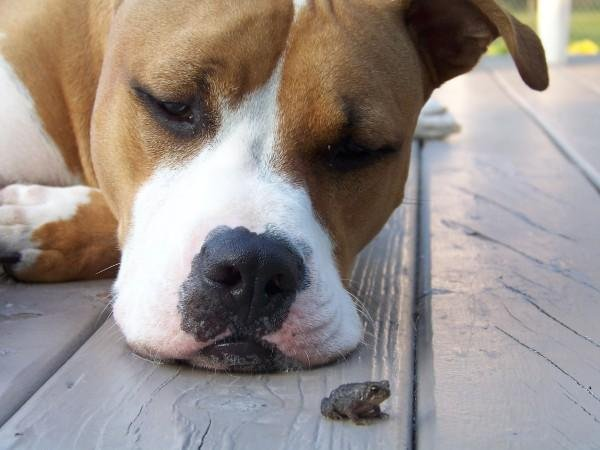
\includegraphics[width=0.5\linewidth]{cachorro} 

}

\caption{Cachorro}\label{fig:unnamed-chunk-11}
\end{figure}

\begin{equation}
y_i=\beta_0 + \beta_1 x_i + \epsilon_i,\label{Eq1}
\end{equation}

Veja equação (\ref{Eq1}).

\end{frame}

\hypertarget{referuxeancias}{%
\section{Referências}\label{referuxeancias}}

\begin{frame}{Referências}
\protect\hypertarget{referuxeancias-1}{}

\hypertarget{refs}{}
\leavevmode\hypertarget{ref-ggplot2}{}%
Wickham, Hadley. 2016. \emph{Ggplot2: Elegant Graphics for Data
Analysis}. Springer-Verlag New York. \url{http://ggplot2.org}.

\end{frame}

\end{document}
